\chapter{Geología}

Geología física en la formación del ingeniero en Riego y Drenaje, 
la geología explica tres de los cincos factores de formación del suelo, en el modelo de Jenny (material parental, relieve y el tiempo); estudia las unidades geológicas cartográficas, tienen relación con las unidades cartográficas de suelos y de formas terrestres, el conocimiento de las propiedades físicas, químicas y mineralógicas son parte fundamental, para los estudios de mecánica de rocas y suelos.

El conocimiento de la relación geología, formas terrestres, facilita la interpretación de escenas de satélite, las rocas determinan la composición química de las aguas subterráneas, la geología y la geomorfología de una región, ayudarán a localizar el mejor sitio para un embalse.

\begin{definition}[Relieve]
    Elevaciones o desigualdades de la superficie de los terrenos, a diferencia de la topografía, que estudia las características que aparecen en un mapa topográfico
\end{definition}

Las formas terrestres (geoformas) son la base para: 
\begin{itemize}
    \item Inventario de recursos naturales,
    \item Unidades de manejo ambiental,
    \item Ordenamiento territorial,
    \item Cartografía de procesos naturales de alto riesgo,
    \item En combinación con la geología, para estudios de aguas subterráneas
\end{itemize}

\section{Minerales}

Una roca es una mezcla heterogénea de uno o más minerales, un mineral es un compuesto químico formado por uno o más elementos químicos.

Para que un compuesto químico sea considerado mineral, debe cumplir con los siguientes requisitos:

\begin{enumerate}
    \item Producto de procesos naturales
    \item Sus átomos deben estar organizados en estructuras regulares
    \item Debe tener composición química (puede variar dentro de ciertos límites)
    \item La composición química debe expresarse mediante una fórmula química
\end{enumerate}

\begin{table}[h!]
    \centering\begin{tabular}{@{}cc@{}}
    \toprule
    Elemento & \begin{tabular}[c]{@{}c@{}}Porcentaje\\ por peso\end{tabular} \\ \midrule
    Oxigeno  & 46.6                                                         \\
    Silicio  & 27.7                                                         \\
    Aluminio & 8.1                                                          \\
    Hierro   & 5.0                                                          \\
    Calcio   & 3.6                                                          \\
    Sodio    & 2.8                                                          \\
    Potasio  & 2.6                                                          \\
    Magnesio & 2.1                                                          \\
    Otros    & 1.7                                                          \\ \bottomrule
    \end{tabular}
    \caption{Abundancia relativa de los elementos más comunes en la corteza terrestre}
    \label{tabg1}
    \end{table}

Algunos compuestos importantes en la geología son los siguientes

\begin{table}[h!]
    \centering\begin{tabular}{@{}cc@{}}
    \toprule
    \begin{tabular}[c]{@{}c@{}}Nombre del\\ Mineral\end{tabular} & \begin{tabular}[c]{@{}c@{}}Composición\\ Química\end{tabular} \\ \midrule
    Olivino                                                      & $(FeMg)2SiO_4$                                                \\
    Ortoclasa                                                    & $KAlSi_3O_8$                                                  \\
    Albita                                                       & $NaAlSi_3O_8$                                                 \\
    Anortita                                                     & $CaAl_2Si_2O_8$                                               \\
    Calcita                                                      & $CaCO_3$                                                      \\
    Halita                                                       & $NaCl$                                                        \\
    Fluorita                                                     & $CaF_2$                                                       \\
    Apatita                                                      & $Ca_5(PO_4)_3(F,Cl,OH)$                                       \\
    Yeso                                                         & $CaSO_4\cdot 2G_2O$                                           \\
    Magnesita                                                    & $MgCO_3$                                                      \\ \bottomrule
    \end{tabular}
    \caption{Composición química de minerales fundamentales en la irrigación y geología}
    \label{tabg2}
    \end{table}
\subsection{Procesos genéticos de minerales}

Existen más de 2,000 especies de minerales pero sólo veinte son minerales formadores de roca

\begin{itemize}
    \item Magmatismo, forma rocas ígneas como las obsidianas, si se enfrían en la superficie de la tierra, se le asigna el nombre de rocas ígneas intrusivas
    \item Intemperismo, forman las arcillas
    \item Sedimentación 
    \item Evaporación
    \item Metamorfismo
\end{itemize}

Minerales de origen magmático:
%%%%%%%%%%%%%%%%%%%%%%%%%%%%%%%%%%%COMPOSICIÖN QUIMICA DE ESTO:
\begin{itemize}
    \item Cuarzo $SiO_2$
    \item Ortoclasa $KAlSi_3O_8$
    \item Anortita $CaAl_2Si_2O_8$
    \item Andesina $(Na,Ca)(Si,Al)_4O_8$
    \item Moscovita $KAl_2(AlSi_3O_{10})(OH)_2$
    \item Biotita $ K(Mg,Fe)_3(AlSi_3O_{10})(F,OH)_2$
    \item Olivino $(Mg,Fe)_2SiO_4$
    \item Piroxena $(Ca,Mg,Fe,Mn,Na,Li)(Al, Mg, Fe, Mn,Cr,Sc,Ti)(Si, Al)_2O_6$
    \item Anfíbola 
    \item Magnetita $FeFe_2O_4 (Fe_2+Fe_3+2 O_4), Fe_3O_4$
\end{itemize}

Minerales de origen intemperismo secundarios:
\begin{itemize}
    \item Arcillas
    \item Óxidos
    \item Hidróxidos
\end{itemize}
Minerales de origen de sedimentación:
\begin{itemize}
    \item Calcita $CaCO_3$
    \item Dolomita $(CaMg(CO_3)_2)$
\end{itemize}
Minerales de evaporación:
\begin{itemize}
    \item Halita $NaCl$
    \item Yeso $ CaSO_4\cdot 2H_2O$
    \item Anhidrita $CaSO_4$
    \item Carnalita $ KMgCl_3\cdot 6H_2O$
\end{itemize}
Minerales de metamorfismo

\begin{itemize}
    \item Granate $(Ca,Fe,Mg,Mn)_3(Al, Fe, Mn,Cr,Ti,V)_2(SiO_4)_3$
    \item CLorita $(Mg,Fe)_3(Si,Al)_4O_{10} (OH)_2\cdot (Mg,Fe)_3(OH)_6$
    \item Talco $Mg_3Si_4O_{10}(OH)_2$
    \item Corundo $Al2O3$
    \item Grafito $C$
    \item Diamante $C$
    \item Wollastonita $Ca(SiO_3)$
    \item Micas 
    \begin{itemize}
        \item Lepidolita $K(Li,Al)_3 (AlSi_3O_{10}) (O, OH, F)$
        \item biotita $K (Mg,Fe)_3 (AlSi_3O_{10})(OH)$
        \item flogopita $KMg_3(AlSi_3O_{10})(OH)$
        \item moscovita $KAl_2(AlSi_3O_{10})(OH)_2$
    \end{itemize}
\end{itemize}

Para observar minerales en el suelo, es preciso pesar 100 gr de suelo, colocarlo en un vaso de precipitados, agregar 10 mililitros de agua oxigenada, mezclar,
agregar agua hasta el borde, agitar fuertemente por 20 segundos y dejar reposar por un minuto. Decantar en una cubeta el agua; Repetir la operación anterior, hasta que el agua después del minuto, esté clara. Finalmente dejar secar al sol

Los silicatos, nesosilicatos (Olivino), Inosilicatos (Piroxenos, enstatita, anfíboles, hornblenda); Filosilicatos, Mica, Biotita tiene de mayor a menor temperatura de formación, mientras que la Plagocioclasa Cálcica, Anortita; Plagioclasa Sódica tienen de menor a mayor

Minerales máficos (Color oscuro):
\begin{itemize}
    \item Olivino
    \item Piroxenos 
    \item Micas
\end{itemize}

Minerales félsicos (Color claro)

\begin{itemize}
    \item Plagioclasas 
    \item Feldespatos 
    \item Cuarzo
\end{itemize}


\begin{table}[h!]
    \centering\begin{tabular}{@{}ccccc@{}}
    \toprule
    Mineral                                                         & Fórmula Química           & Estructura                                                            & \begin{tabular}[c]{@{}c@{}}Respuesta al\\ Intemperismo\end{tabular}                    & Producto                                                      \\ \midrule
    Cuarzo                                                          & $SiO_2$                   & Tectosilicato                                                         & \begin{tabular}[c]{@{}c@{}}Permanece sin\\ descomponerse\end{tabular}                  & \begin{tabular}[c]{@{}c@{}}Granos de\\ cuarzo\end{tabular}    \\
    Ortoclasa                                                       & $KAlSi_3O_8$              & Tectosilicato                                                         & \begin{tabular}[c]{@{}c@{}}Entra en solución, con\\ liberación de silicio\end{tabular} & Arcillas                                                      \\
    Muscovita                                                       & $KAl_2(AlSi_3O_{10})(OH)$ & Filosilicato                                                          & \begin{tabular}[c]{@{}c@{}}Permanece sin\\ descomponerse\end{tabular}                  & \begin{tabular}[c]{@{}c@{}}Escamas de\\ micas\end{tabular}    \\
    Apatita                                                         & $Ca_3(PO_4)_2(FCl)$       & No es silicato                                                        & Soluble                                                                                & \begin{tabular}[c]{@{}c@{}}Material\\ soluble\end{tabular}    \\
    Olivino                                                         & $(Mg,Fe)_2SiO_4$          & Nesosilicato                                                          & \begin{tabular}[c]{@{}c@{}}Soluble, formación de\\ óxido e hidróxidos\end{tabular}     & \begin{tabular}[c]{@{}c@{}}óxidos e\\ hidróxidos\end{tabular} \\
    \begin{tabular}[c]{@{}c@{}}Piroxeno\\ (Hiperstena)\end{tabular} & $(Mg,Fe)SiO_3$            & \begin{tabular}[c]{@{}c@{}}Inosilicato de\\ cadena doble\end{tabular} & \begin{tabular}[c]{@{}c@{}}Soluble, formación de\\ óxidos e hidróxidos\end{tabular}    & \begin{tabular}[c]{@{}c@{}}óxidos e\\ hidróxidos\end{tabular} \\
    Anortita                                                        & $CaAl_2Si_2O_8$           & Tectosilicato                                                         & Entra en solución con liberación de silicio                                            & Arcillas                                                      \\
    Magnetita                                                       & $Fe_2O_3$                 & No es silicato                                                        & Formación de óxidos                                                                    & \begin{tabular}[c]{@{}c@{}}óxidos e\\ hidróxidos\end{tabular} \\ \bottomrule
    \end{tabular}
    \caption{Roca granito (Primeros cinco) y Roca basalto (últimos cinco)}
    \label{tabg3}
    \end{table}

\begin{figure}[h!]
    \centerline{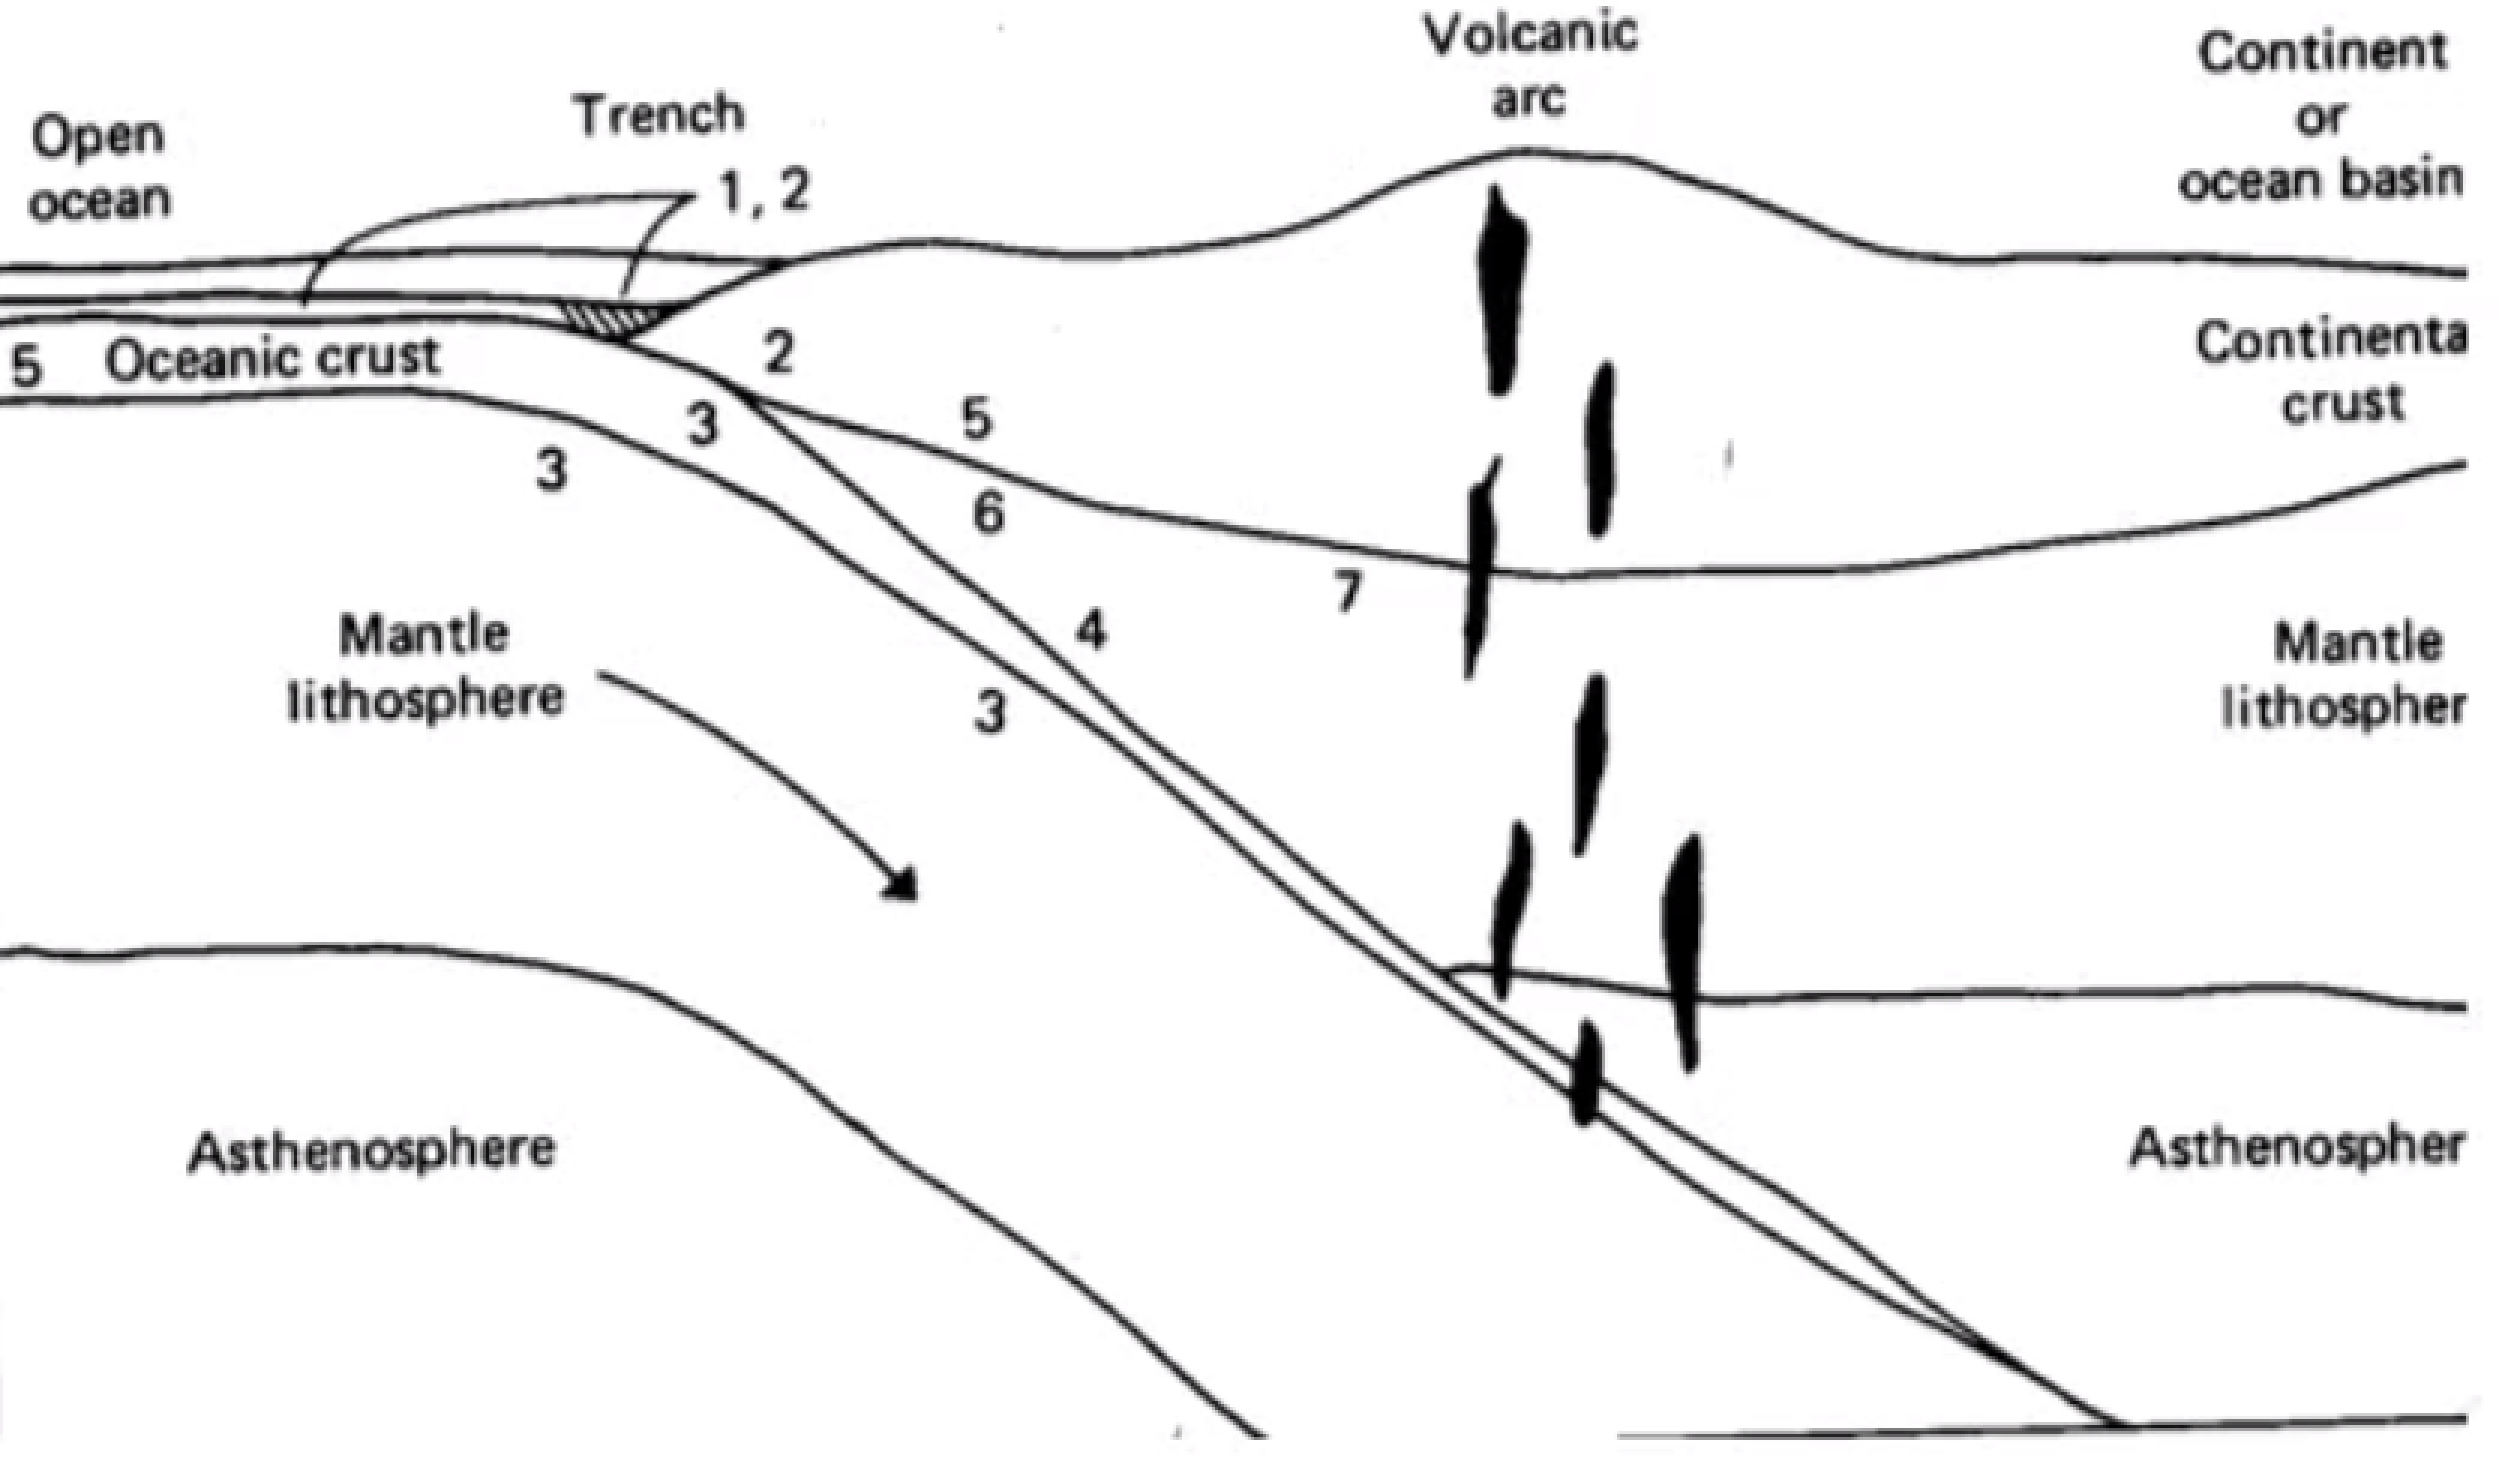
\includegraphics[width=0.5\textwidth]{g1.png}}
    \caption{Formación de las rocas ígneas}
    \label{g1}
\end{figure}

\begin{definition}[Arcilla]
    En ingeniería Civil, se define como material plástico derivado de las rocas, en mineralogía son minerales con una estructura de tetraedros y octaedros, pero en geología es material con granulometría menos de dos milímetros, equivalente a barro.
\end{definition}

Se hallan $6OH^-$ molecularmente, así que se necesitan seis cargas positivas para neutralizar la capa octaédrica de la arcilla.

\begin{itemize}
    \item Brucita $Mg3(OH)_6$
    \item Gibbsita $Al2(OH)_6$
\end{itemize}

\begin{enumerate}
    \item Caolinita
    \item Montmorillonita
    \item Illita 2:1:1
\end{enumerate}

\begin{table}[h!]
    \centering\begin{tabular}{@{}cccc@{}}
    \toprule
    Propiedad                                                                                       & Montmorillonita                                                                          & Illita                                                                               & Caolinita                                                       \\ \midrule
    Estructura                                                                                      & Celosía 2: 1                                                                             & Celosía 2: 1                                                                         & Celosía 1: 1                                                    \\
                                                                                                    & \begin{tabular}[c]{@{}c@{}}Sustitución en\\ hojas octaédricas\\ por Mg o Fe\end{tabular} & \begin{tabular}[c]{@{}c@{}}Sustitución en\\ hojas tetraédricas\\ por Al\end{tabular} & \begin{tabular}[c]{@{}c@{}}No hay\\ sustitución\end{tabular}    \\
    Forma                                                                                           & Copos irregulares                                                                        & Copos irregulares                                                                    & \begin{tabular}[c]{@{}c@{}}Cristales\\ hexagonales\end{tabular} \\
    \begin{tabular}[c]{@{}c@{}}Área total\\ de superficie\\ ($m^2/g$)\end{tabular}                  & 700-800                                                                                  & 100-120                                                                              & 5-20                                                            \\
    \begin{tabular}[c]{@{}c@{}}Cohesión\\ Plasticidad y\\ capacidad de \\ hinchamiento\end{tabular} & Alto                                                                                     & Medio                                                                                & Bako                                                            \\
    \begin{tabular}[c]{@{}c@{}}Superficie externa\\ Superficie interna\end{tabular}                 & 80-100                                                                                   & 15-40                                                                                & 3-15                                                            \\
    \begin{tabular}[c]{@{}c@{}}Capacidad de \\ intercambio catiónico\end{tabular}                   & 80-100                                                                                   & 15-40                                                                                & 3-15                                                            \\
    \begin{tabular}[c]{@{}c@{}}Capacidad de \\ intercambio iónico\end{tabular}                    & Bajo                                                                                     & Medio                                                                                & Alto                                                            \\ \bottomrule
    \end{tabular}
    \caption{Comparación de las propiedades de minerales de arcilla de silicato}
    \label{tabg4}
\end{table}


\begin{definition}[Rocas ígneas]
    Son aquellas que se formaron por la cristalización de un magma
\end{definition}

Se pueden clasificar por dos criterios, el primero es el contenido de silicio $SiO_2$
óxidos que componen a todas las rocas:
\begin{align*}
    &SiO_2&&CaO&&H_2O^+&&K_2O\\
    &Fe_2O_33&&Na_2O&&H_2O^-\\
    &FeO&&Al_2O_3&&P_2O_5\\
    &MgO&&MnO&&TiO_2
\end{align*}

El porcentaje de óxido de silicio, se ve reflejado en el color de la roca.

\begin{itemize}
    \item más de 66\% de volumen de $siO_2$ de la roca \textbf{sílicas}
    \item Color claro: Gris claro, blanco y roca
    \item Otro grupo es 66 y 55\% de la roca \textbf{subsílicas}
    \item Color: gris, rojo y verde
    \item El último está entre 55 y 45\% de la roca \textbf{asílica}
    \item Colos obscuro: gris oscuro, y negro
    \item Menos de 45\% ultrabásicas
\end{itemize}

El lugar de enfriamiento (cristalización) del magma, \textit{Intrusivas} si el magma se cristaliza en el interior de la corteza terrestre (más de tres kilómetros de profundidad)

\begin{definition}[Porfídicas]
    El magma, al fluir hacia la superficie, entra en contacto con las rocas que va penetrando y va perdiendo energía calorífica, se cristalizan los primeros minerales, al extrusionar completamente el resto del magma que permanecía fluyendo, se cristaliza rápidamente, éste proceso forma cristales grandes y cristales microscópicos.
\end{definition}

\begin{table}[h!]
    \centering\begin{tabular}{@{}llll@{}}
    $\%SiO_2$ Textura                                                & \begin{tabular}[c]{@{}l@{}}Afanitica\\ (fina)\end{tabular} & \begin{tabular}[c]{@{}l@{}}Porfídica\\ (intermedia)\end{tabular} & \begin{tabular}[c]{@{}l@{}}Fanerítica\\ (gruesa)\end{tabular} \\
    \begin{tabular}[c]{@{}l@{}}Silicas\\ ácidas\end{tabular}         & Riolita                                                    & \begin{tabular}[c]{@{}l@{}}Porfido\\ riolítico\end{tabular}      & Granito                                                       \\
    \begin{tabular}[c]{@{}l@{}}Subsílicas\\ intermedias\end{tabular} & Andesita                                                   & \begin{tabular}[c]{@{}l@{}}Porfido\\ andesítico\end{tabular}     & diorita                                                       \\
    \begin{tabular}[c]{@{}l@{}}Asílicas\\ básicas\end{tabular}       & Basalto                                                    & \begin{tabular}[c]{@{}l@{}}Dolerita ó\\ Diabasa\end{tabular}     & Gabro                                                        
    \end{tabular}
    \caption{Identificación de rocas ígneas}
    \label{tabg5}
\end{table}

Los sedimentos pueden ser fragmentos de rocas y/o minerales (terrígenas), o de compuestos químicos

\begin{definition}[Rocas metamórficas]
    Rocas que son producto de cambios mineralógicos y tecturales, ocasionados por cambios de temperatura, presión y circulación de soluciones químicas a altas temperaturas (hidrotermales)
\end{definition}

El aumento de temperatura se debe al contacto con intrusivos ígneos y aumento de la presión por sepultamiento; La principal causa de aumento de la presión es el sepultamiento. También se debe a las soluciones químicas a altas temperaturas, al enfriarse el magma, los gases disueltos, atraviesan las  rocas confinantes, cambiándose con los minerales de esas rocas, también subiendo la temperatura para que los minerales se recristalicen. El proceso de recristalización de los minerales, siempre es en estado sólido, se llegase a fundir la roca, sería ígnea, esto se refleja en la textura

La presión, de forma parecida a la temperatura, también se incrementa con la profundidad, se incrementa en 1kbar por cada 4.4 kilómetros.

Mientras que los fluidos hidrotermales, se componen de agua y otros compuestos volátiles, tal como dióxido de carbono, el agua actúa como un catalizador durante el metamorfismo. El agua ayuda el cambio de iones entre cristales de minerales. Las soluciones hidrotermales originan los yacimientos de minerales de rendimiento económico.

\subsection{Intemperismo}

Es un proceso geológico de origen externo (en la superficie de la tierra) mediante las cual las rocas se adaptan a las nuevas condiciones de presión y temperatura

\subsubsection{Intemperismo físico}

Se caracteriza éste intemperismo por reducir de tamaño y volumen a las rocas, no hay reacciones químicas.

Actúa por los siguientes mecanismos; Cambios de temperatura, acción de la cuña de hielo y cristalización de sales.

\textbf{Cambios de temperatura}, los minerales que forman a las rocas son de diversos colores, por lo que tendrán diferente captación de radiación solar, los minerales máficos se calentará más durante el día, tendrán mayor dilatación, los minerales félsicos tienen menor dilatación.

En los desiertos se ha medido la temperatura durante todo el día, registrándose temperaturas de hasta $54^{\circ}C$ a las dos de la tarde y de $-10^{\circ}C$ durante noche (Embleton, 1979). Estos cambios de temperatura provocan que el mineral durante el día se dilate en cierta proporción y durante la noche se contraiga, haciendo que los minerales se rompan después de un tiempo

Este mecanismo del intemperismo se presenta en aquellas regiones en las que las diferencias de temperatura, entre el día y la noche, son significativas y no solamente en el desierto.

\textbf{Acción de la cuña del hielo.}

Casi todos hemos observado, que cuando dejamos en el congelador un recipiente con agua, al cabo de unos días, el recipiente se ha roto por la acción de la formación de hielo en su interior. Esto se debe a que el agua incrementa en 9\% su volumen durante su cambio a hielo. Genera una fuerza de 2000 $lb/pg^2$, si se compara esta fuerza con la necesaria para quebrar un bloque de granito, de dos pulgadas de espesor, 600 $lb/pg^2$, se observará que el agua cuando se congela, podrá romper casi cualquier material.

Este mecanismo se presenta en aquellas regiones donde la temperatura baja a $4^{\circ}C$ o menos

\textbf{Cristalización de Sales.}

Este mecanismo se produce por la humedad presente en las rocas, principalmente en la capa superficial, la presencia de algunas sales dentro del agua, provoca que al evaporarse ésta, las sales se precipitan paralelamente a la superficie de la roca, rompiéndola en escamas(Loughnan1969).

Muchas sales, de calcio, sodio, magnesio, potasio y bario, tienen alto coeficiente de expansión volumétrica. Sus volúmenes se incrementan con la temperatura y su expansión puede ser tres veces más que la del granito en condiciones similares.

Durante el día, con las altas temperaturas, los cristales de las sales formados, que están bajo la capa superficial

de las rocas crecen.

El intemperismo físico se presenta en las regiones con precipitaciones menores de 700 mm. Su principal producto son fragmentos de roca.

\subsubsection{Intemperismo químico}

La característica de este proceso es la formación de nuevos minerales, por reacciones químicas de los minerales de las rocas con el agua y el dióxido de carbono.

La molécula del agua consiste de un átomo de oxígeno y dos de hidrógeno, enlazados covalentemente. La molécula es dipolar, por lo que, el enlace es asimétrico. Los átomos de hidrógeno tienen una carga neta positiva y los átomos de oxígeno una doble negativa. Esta estructura favorece el enlace iónico entre los átomos de hidrógeno, en grupos tetraédricos para cuatro moléculas y le da la propiedad de una alta superficie de tensión y fuerza de tensión. adhesión y capilaridad (Embleton, 1979).

Las reacciones químicas del intemperismo son exotérmicas.

Las principales reacciones que pueden ocurrir, durante el intemperismo químico, son las siguientes;

\textbf{Oxidación y Reducción}

Entendemos la oxidación y la reducción como la ganancia o pérdida de oxígenos. Una reacción típica de oxidación es la siguiente;

\begin{equation}
    4Fe3O4+ O_2 \longrightarrow  6Fe_2O_3
\end{equation}

En esta reacción la Magnetita en presencia de oxígeno, forma Hematita.

Las reacciones de oxidación, también, se pueden llevar a cabo en presencia de agua;

\begin{equation}
    FeS + HO + 15O \longleftrightarrow  2FeO + 16H^+ +85O^{- 2}
\end{equation}

pirita

Las \textbf{reacciones de oxidación}, se presentan en ambientes donde hay circulación del oxígeno, mientras que, las de reducción, se presentan en ambientes donde el oxígeno no circula libremente, por ejemplo, en el fondo de los cuerpos de agua.

Los productos de la oxidación, generalmente presentan colores rojizos, como el de la hematita, los productos de la reducción presentan colores gris verdoso. Al hacer una cata de suelos, en regiones, donde antes hubo un cuerpo de agua por un largo tiempo, encontramos un horizonte de color verdoso, llamado horizonte gley.

\textbf{Hidrólisis}

En esta reacción, el agua, se comporta como un separador eléctrico con sus polos positivo, el hidrógeno y negativo, el oxígeno.

En los silicatos, la hidrólisis consiste en la ruptura de la estructura cristalina por el enlace iónico que une a los cationes Na, K, Mg, Ca, y Fe, con los aniones $AlSi_30_8$, $Al_2Si_2O_8$, $SiO_3$ y $4+ SO_4$, el catión $H$ reemplaza a los cationes y estos entran en solución en equilibrio con los aniones $OH^-$, $CO_2$ Y $HCO^-$ (Loughnan, 1969).

\textbf{Carbonatación}

Esta reacción se efectúa por la combinación del ácido carbónico con los minerales para formar bicarbonatos o carbonatos. Se lleva a cabo principalmente sobre las rocas calizas de acuerdo a la siguiente reacción;
\begin{equation}
    Caliza:\, H_2O + O_2 \longrightarrow > Ca^{ + 2} + 2HCO^ -
\end{equation}

\textbf{Acción directa}

Los agentes de éste intemperismo son los organismos principalmente plantas. Las raíces agrietan las rocas, se fragmentan y después por medio de los pelos absorbentes, descomponen los minerales, de los cuales toman sus nutrientes.

\textbf{Acción indirecta}

La llevan a cabo los organismos, al realizar algunas de sus funciones dentro del suelo, tal como la construcción de madrigueras

\section{Tectónica de placas}
De la deriva de los conientes a la tectónica de placas

En 1885, basándose en la distribución de flores fósiles y de sedimentos de origen glacial, el geólogo suizo Suess propuso la existencia de un supercontinente que incluía India, África y Madagascar, posteriormente añadiendo a Australia y a Sudamérica. A este supercontinente se le denominó Gondwana.

El astrónomo y meteorólogo alemán Alfred Wegener (1880-1930) fue quien propuso que los continentes en el pasado geológico estuvieron unidos en un supercontinente de nombre Pangea, que posteriormente se habría disgregado por deriva continental.

Su libro Entstehung der Kontinente und Ozeane (La Formación de los Continentes y Océanos; 1915) tuvo poco reconocimiento y fue criticado por falta de evidencia a favor de la deriva, por la ausencia de un mecanismo que la causara, y porque se pensaba que tal deriva era físicamente imposible.

En 1937, el geólogo sudafricano Alexander Du Toit publicó una lista de diez líneas de evidencia a favor de la existencia de dos supercontinentes, Laurasia y Gondwana, separados por un océano de nombre Tethys el cual dificultaría la migración de floras entre los dos supercontinentes. Du Toit también propuso una reconstrucción de Gondwana basada en el arreglo geométrico de las masas continentales y en la correlación geológica.
Evidencia de un evento glacial pérmico (hace 280 millones de años) han sido reportados en Sudamérica, África, India, Australia y Antártida. En las reconstrucciones de Gondwana, las áreas afectadas por la glaciación son contiguas a pesar de ocupar lo que hoy en día son distintos continentes. Inclusive las direcciones de flujo del hielo, obtenidas a partir de las marcas de abrasión, son continuas de África occidental a Brasil y Argentina así como lo son de Antártida a India

Las distribuciones de rocas cristalinas, rocas sedimentarias y yacimientos minerales forman patrones que continúan ininterrumpidos en ambos continentes cuando Sudamérica y África son restituidos cerrando el océano Atlántico.

Estudios de la distribución de plantas y animales fósiles también sugieren la existencia de Pangea. Impresiones de hojas de un helecho, Glossopteris, están ampliamente distribuidas en rocas de África, Sudamérica, India y Australia

En los años 30 el geofísico japonés Wadati documentó el incremento en la profundidad de los sismos en función de la distancia tierra adentro hacia el continente. Al mismo tiempo el sismólogo Hugo Benioff documentaba la misma variación y resaltaba el hecho de que las zonas de alta sismicidad no estaban distribuidas de manera uniforme sobre el globo terráqueo, sino que éstas se alojaban en fajas más o menos continuas asociadas a algunas márgenes continentales.
\begin{figure}[h!]
\centering
  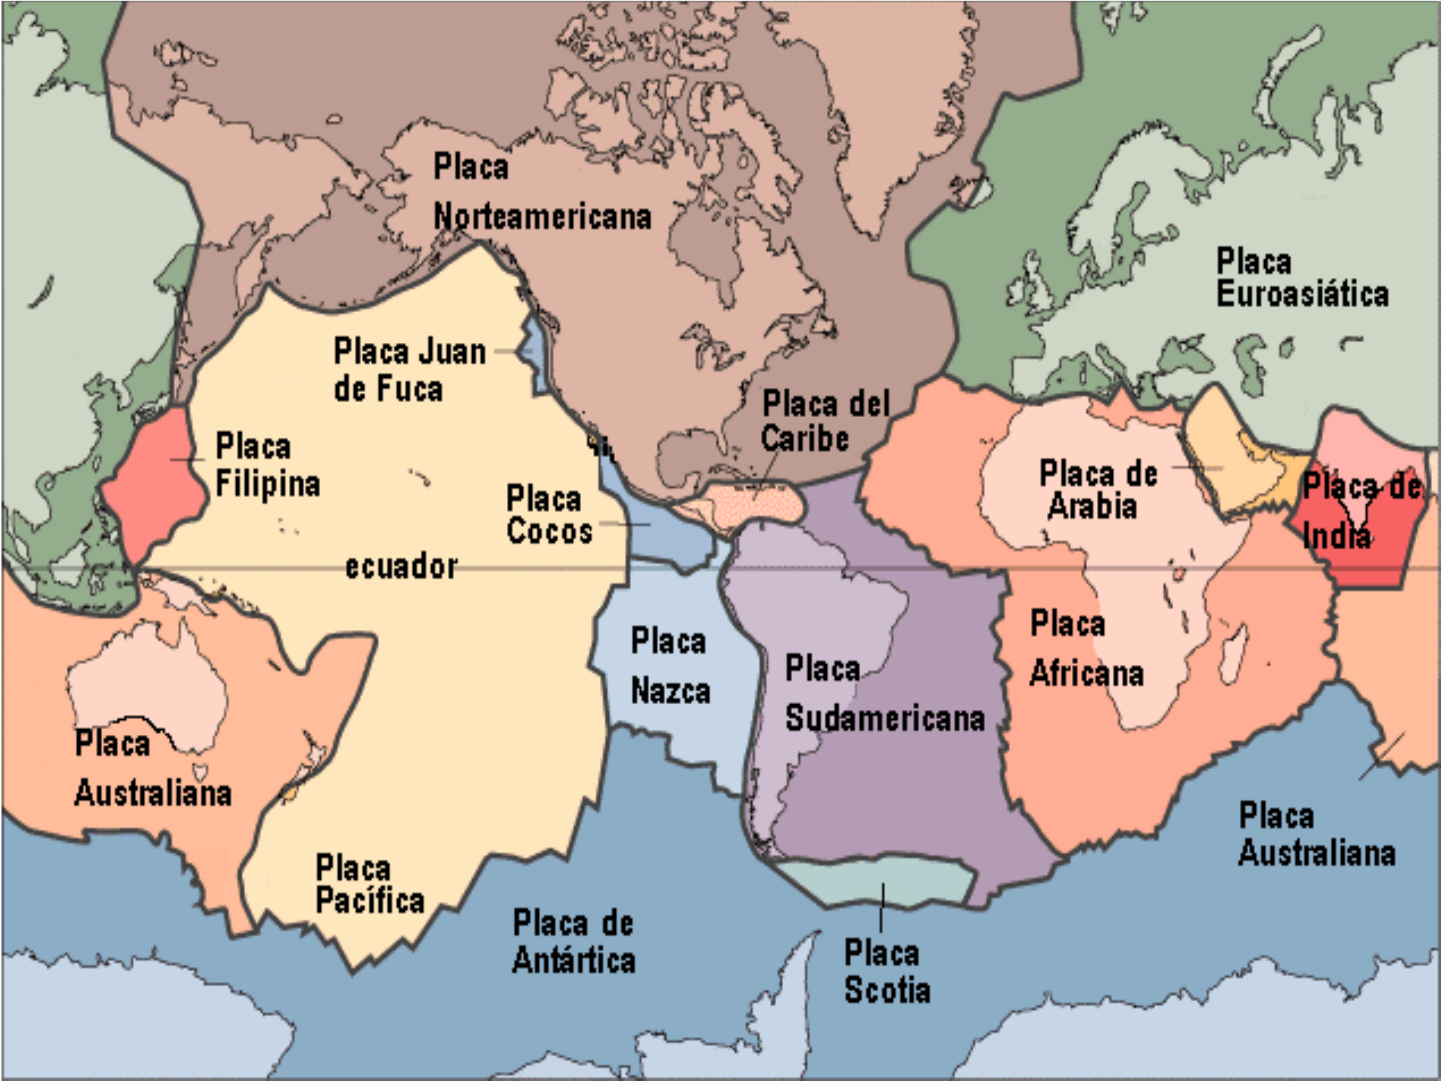
\includegraphics[width=0.5\textwidth]{g4.png}
  \caption{Tectónica global}
  \label{g4}
\end{figure}
A principios de los años 60 el geofísico H.H. Hess sugirió un mecanismo que podría explicar la deriva continental, basándose en las variaciones topográficas de los océanos

Hess propuso que las rocas de los fondos marinos estaban firmemente ancladas al manto que les subyacía. Conforme se apartaban dos enormes masas de manto, acarreaban pasivamente el fondo oceánico y surgía de las profundidades terrestres material fundido que formaba una cadena volcánica y que rellenaba el vacío formado por la separación de los fondos oceánicos. Si esto fuera cierto, razonó Hess, para evitar un crecimiento indefinido de la Tierra era necesario que en alguna parte de ella fuera consumido material cortical. Propuso entonces que los sitios donde esto ocurría eran las profundas fosas oceánicas que bordeaban algunos continentes y arcos de islas.

Los registros magnetométricos indicaban patrones lineales muy claros de anomalías magnéticas positivas (donde la fuerza magnética era mayor que el promedio) y negativas (donde la fuerza magnética era menor que el promedio). Las anomalías magnéticas eran también simétricas con respecto al eje de la cadena montañosa del fondo marino.
\begin{figure}[h!]
\centering
  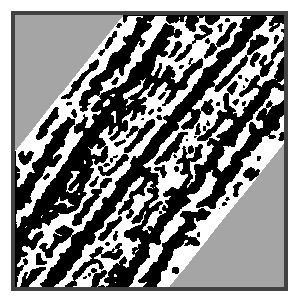
\includegraphics[width=0.5\textwidth]{g3.jpg}
  \caption{Magnetismo}
  \label{g3}
\end{figure}
Esta observación encajaba con la del francés Bernard Bruhnes, quien en 1906 había propuesto que el campo magnético terrestre se invertía más o menos cada medio millón de años. Vine y Matthews concluyeron que las rocas volcánicas de los fondos marinos estaban registrando la polaridad del magnetismo terrestre en el momento de su cristalización; conforme se invertía esta polaridad cada 500,000 años, las rocas que se formaban constantemente en las dorsales oceánicas iban registrando los cambios de polaridad. De esta manera propusieron que la anchura de las franjas magnéticas debería ser igual a la velocidad de separación de las placas, multiplicada por la duración del intervalo de tiempo entre inversiones de polaridad.

Alfred Wegener en 1912, que todavía se debatía acaloradamente, sobre todo en la universidades británicas y australianas, gracias al texto de 1945 Principles of Physical Geology de Arthur Holmes.

Jason Morgan y Dan Mckenzie, en 1967 y 1968 respectivamente. Ambos proponían que placas rígidas, cada una de ella de aproximadamente 100 km de espesor, cubrían la superficie de la Tierra. Eran estas placas, y no las montañas o los océanos, las características estructurales verdaderamente importantes de la superficie de la Tierra.

\section{ArcMap 10.8}

El ArcGIS está compuesto por tres productos principales: ``ArcMap'', ``ArcToolbox''. ``ArcCatalog''.
\textbf{ArcCatalog}. Herramienta para organizar y documentar los datos geográficos (metadata). Los datos pueden ser movidos, copiados, borrados y se pueden previsualizar antes de agregarlos al mapa. Los metadatos, pueden ser creados, editados o leídos.

\textbf{ArcToolbox}. Es un conjunto de herramientas que se utilizan para el geoprocesamiento: Combinar capas, manipulación de los datos, definición y transformación de sistemas de coordenadas. 

\textbf{ArcMap}. Es la principal aplicación de ArcGIS, que es usada para la entrada de datos, edición análisis estadístico y geográfico, además se pueden generar salidas, como mapas impresos. ArcMap incluye un conjunto de barras de herramientas para trabajar con mapas y su contenido. Dichas barras de herramientas se usan para navegar por los mapas (ej. zoom y seleción), editar características y generar mapas para impresión.

ArcCatalog es un programa independiente de ArcMap (en la versión 10 viene integrado en ArcMap), que permite organizar (copiar, pegar, mover, definir proyecciones, etc.) y editar metadatos, de la información geográfica para uso en los programas de ArcGIS. También permite conexión a discos o servidores remotos.

El principal formato para almacenar información geográfica de tipo vector, es el \textit{shape}. Un shape está compuesto por tres archivos: 
\begin{itemize} 
    \item .shp : Almacena información sobre forma y localización de un elemento. 
    \item .dbf : Es un archivo de base que almacena los atributos del elemento. 
    \item .shx : Almacena el índice de correspondencia entre la geometría de un elemento y su registro correspondiente en la base de datos. 
\end{itemize}
Todos los archivos antes mencionados son indispensables para que se pueda trabajar la capa en ArcGIS, si alguno de ellos falta, el mapa no se podrá cargar.




























































%\section{Rocas ígneas}
%
%\section{Procesos geológicos externos}
%
%\section{Procesos geológicos internos}
%
%\section{Métodos geofísicos de exploración}
%
%\section{Geología aplicada}

